\documentclass[12pt]{../notes}

% Command for Questions
%\question{}

% Command for Notes
% \note{}

% Code to create a minipage where you can type in class notes. 
%%\begin{minipage}[l][2cm][c]{\textwidth}
%\begin{comment}

%\end{comment}
%%\end{minipage}

%\usepackage{listings}

% In order for the minted code to run, we had to create a new compilation routine called pdflatex+shellEscape.
% This includes a --shell-escape command which should ONLY be used when pygmentized is required as it compromises security. 
% We also had to add pygmentize (a python package) to the system path (BEFORE miktex) and then restart the computer. 
%\usepackage{minted}
%\usemintedstyle{borland}
%\lstset{language=SAS, 
 % breaklines=true,  
 % basicstyle=\ttfamily\bfseries,
  %columns=fixed,
  %keepspaces=true,
  %identifierstyle=\color{blue}\ttfamily,
  %keywordstyle=\color{cyan}\ttfamily,
  %stringstyle=\color{purple}\ttfamily,
  %commentstyle=\color{green}\ttfamily,
  %} 
  
% \begin{minted}{sas}
% \end{minted}

\usepackage{hyperref}


% Begin Document
%==============================================================================
\begin{document}
% Include the Title of the Handout
\ntitle{7.1: Generalized Additive Models (GAM)}

\section{Why GAMs?}

Up to this point we have assumed models of the form 
%
\begin{equation*}
E\left(Y|X_1, X_2, \ldots , X_{p-1}\right) = \beta_0 + \beta_1X_1 + \beta_2X_2 +\cdots + \beta_{p-1}X_{p-1} 
\end{equation*}
%
which quickly fail if the effects cannot be modeled linearly (with possible variable transformations). 

\nspace
As with LOESS regression, GAMs do not assume a particular model form. GAMs only assume that the effects of each variable are additive (no interactions) i.e. 
%
\begin{equation*}
E\left(Y|X_1, X_2, \ldots , X_{p-1}\right) = \beta_0 + f_1(X_1) + f_2(X_2) +\cdots + f_{p-1}(X_{p-1}) 
\end{equation*}
%
where $f_k$ is some unknown function that relates $X_k$ to $Y$.

\nspace
In practice, $f_k$ are approximated using \textbf{cubic smoothing splines}, though any smoothing strategy will do. Splines are preferred because they are computationally much more efficient than weighted regression (as is used in LOESS). The key is that the smoothing occurs \textit{over one dimension at a time} after accounting for the effects of the other dimensions.  

\section{Fitting GAMs}

\subsection{Splines}

\textbf{Splines} are a series of piecewise polynomials that is continuous and differentiable at the break points, called \textbf{knots} (see Figure \ref{fig:spline_example}).

\begin{figure}[H]
\centering
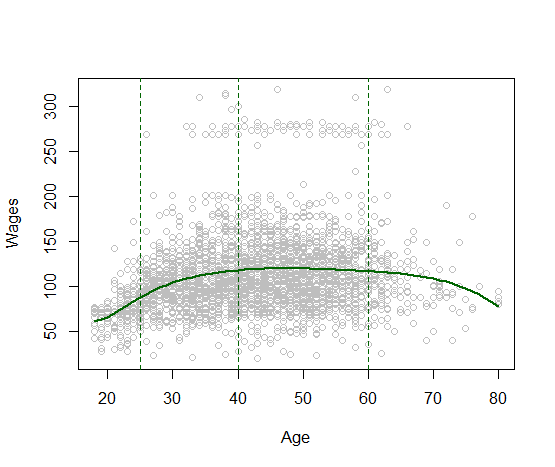
\includegraphics[width = 0.5\textwidth]{../figures/module7/spline_example.png}
\caption{Example of cubic spline with three knots. Code to create image taken from \url{https://datascienceplus.com/cubic-and-smoothing-splines-in-r/}.}
\label{fig:spline_example}
\end{figure}

\nspace
The more knots, the more ``wiggly'' your data has the chance to become. 

\nspace
\textbf{Smoothing Splines} place a knot at every unique value of X. This will most certainly lead to overfitting, so the splines are constrained by an \textit{effective} degrees of freedom to prevent this. The effective degrees of freedom is often selected via \textbf{cross validation}. 

\nspace 
The best part about smoothing splines is that it eliminates the need to select the placement of the knots. 

\subsection{Fitting GAMs}
Remember that we have a unique smoothing spline that relates each X to Y after accounting for the effects of all other X's. 

Hastie et al. (2002) outlines the algorithm for fitting GAMs

\begin{enumerate}
\item Set $b_0 = \bar{y}$ and all $\hat{f}_j \equiv 0$.
\item Cycle through all possible values for $j$ each time updating predictions as:
\begin{itemize}
\item Fit a smoothing spline $S_j$ to the points $(x_{ij}, y_j)$ after accounting for the effect of all other explanatory variables i.e. 
\begin{equation*}
\hat{f}_j \leftarrow S_j\left[\left\{y_i - b_0 - \sum_{k \ne j}\hat{f}_k(x_{ik})\right\}^N_1\right]
\end{equation*}
\item To account for machine imprecision, recenter the splines around 0 i.e.
\begin{equation*}
\hat{f}_j \leftarrow \hat{f}_j  - \frac{1}{N}\sum_{i=1}^N \hat{f}_j(x_{ij})
\end{equation*}
\end{itemize} 
\item Repeat Step 2 until the predicted values of $\hat{f}_j$ stop changing (or change very little). 
\end{enumerate}

\section{Comparisons to Other Methods}

\subsection{LOESS}
\begin{itemize}
\item GAMs using splines are much more computationally efficient than LOESS. 
\begin{itemize}
\item Splines fit models to ``chunks'' of data, while LOESS uses weighted least squares on moving neighborhoods of data. 
\item The sliding window requires continually recalculating distances between points in LOESS, which does not scale well to large datasets. 
\end{itemize}
\item GAMs fit smoothing curves to each variable individually, while LOESS fits one weighted regression surface to all explanatory variables at the same time. 
\item LOESS is great for one to two dimensional smooths on moderate to small datasets. GAMs are better suited for high dimensional data on large datasets. 
\end{itemize}

\subsection{OLS}
\begin{itemize}
\item Both GAMs and OLS are easy to explain to other people (GAM effects are easy to visualize). 
\item GAMs do not require linearity like OLS. 
\item GAMs more computationally expensive to fit compared to OLS. 
\item GAMs can suffer from instability if the data is sparse at the endpoints. 
\end{itemize}


\section{Good Resources}
\bi
\item Hastie, Trevor, Tibshirani, Robert, and Friedman, Jerome (2001) “The Elements of Statistical Learning” (Chapter 9) \url{https://web.stanford.edu/~hastie/Papers/ESLII.pdf}
\ei
% End the Document
%==============================================================================
\end{document}